\section{Evaluering}

\subsection{Test af sensormodeller}
\begin{frame}
\frametitle{Sammenlignings-skema}
\centering
\vspace{-1em}
\begin{tabular}{ l l | c | c | c |}
\cline{3-5}
&&\multicolumn{3}{| c |}{Optimalt}\\\cline{3-5}
&& Optaget&Fri&Ukendt\\\hline

\multicolumn{1}{| l |}{\multirow{3}{*}{Test}}&
Optaget & $+1$ & {\color{red}$-1$} & {\color{gray}$0$}
\\\cline{2-5}

\multicolumn{1}{|c|}{}&
Fri     & {\color{red}$-1$} & $+1$ & {\color{gray}$0$}
\\\cline{2-5}

\multicolumn{1}{|c|}{}&
Ukendt  & {\color{red}$-1$} & {\color{red}$-1$} & {\color{gray}$0$}
 \\\hline
\end{tabular}
\vspace{1em}
\begin{columns}
\begin{column}{.49\textwidth}
\visible<2->{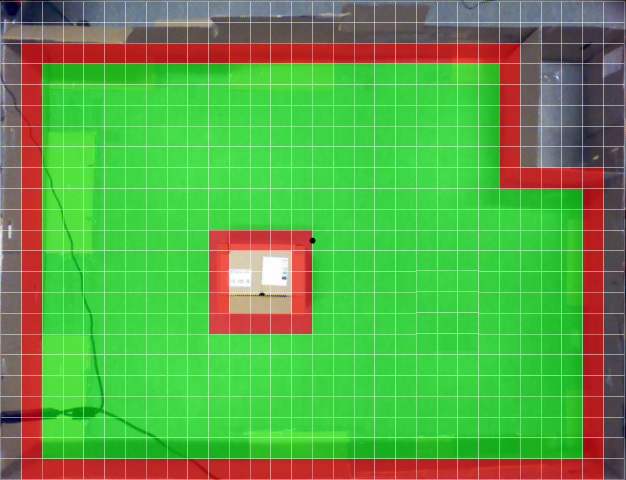
\includegraphics[width=\textwidth]{testresultater/optimalt}}
\end{column}
\begin{column}{.49\textwidth}
\visible<3->{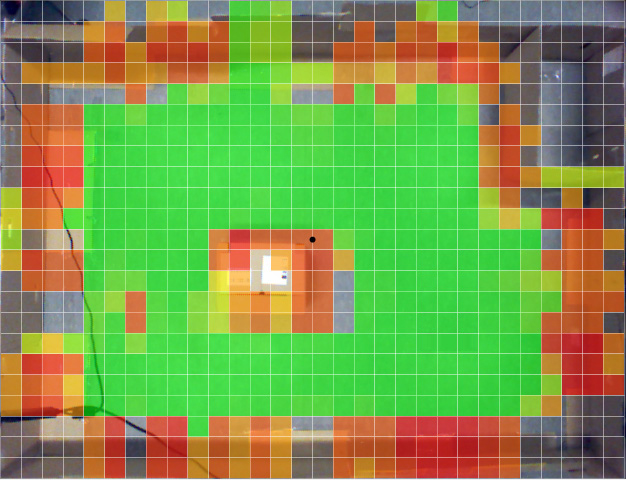
\includegraphics[width=\textwidth]{testresultater/simpel1}}
\end{column}
\end{columns}
\end{frame}


% SIMPEL SENSOR MODEL
\begin{frame}[fragile]{Simpel sensormodel}
	\begin{columns}
		\begin{column}{0.5\textwidth}
			\begin{itemize}
			\item \textbf{100}/150 opdateringer
			\item \textbf{127}/555 point
			\end{itemize}
			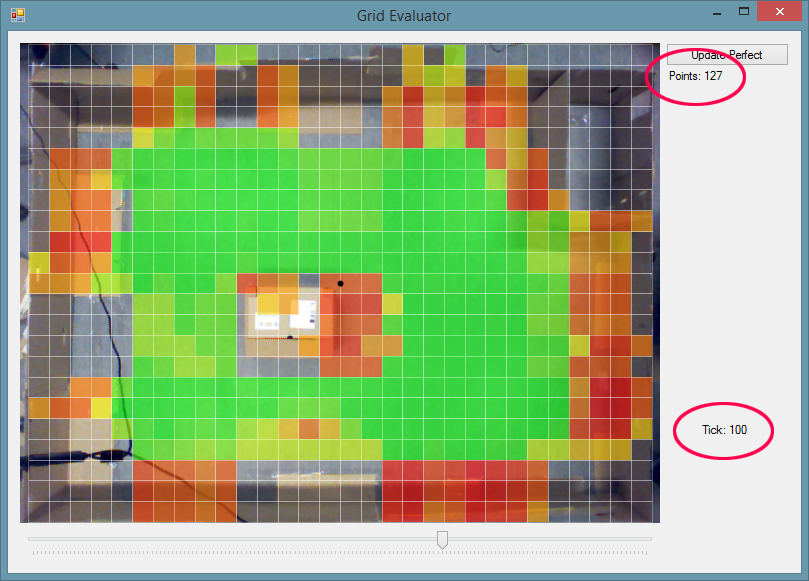
\includegraphics[width=\textwidth]{evaluering/simple3_100.png}
		\end{column}
		\begin{column}{0.5\textwidth}
			\begin{itemize}
			\item \textbf{150}/150 opdateringer
			\item \textbf{193}/555 point
			\end{itemize}
			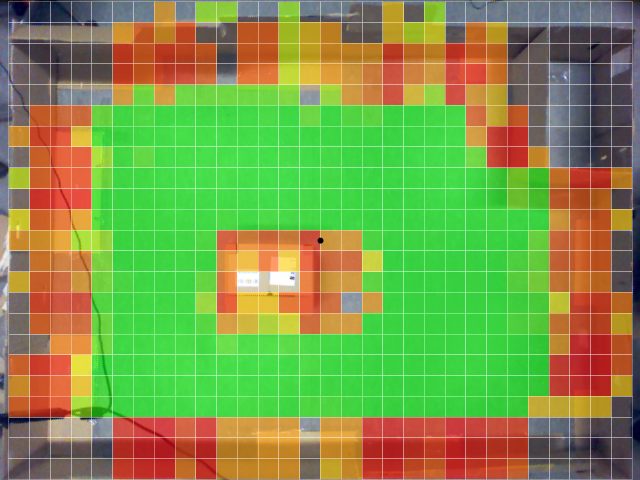
\includegraphics[width=\textwidth]{evaluering/simple3_150.png}
		\end{column}
\end{columns}
\end{frame}

% GAUSISK SENSOR MODEL
\begin{frame}[fragile]{Gausisk sensormodel}
	\begin{columns}
		\begin{column}{0.5\textwidth}
			\begin{itemize}
			\item \textbf{100}/150 opdateringer
			\item \textbf{295}/555 point
			\end{itemize}
			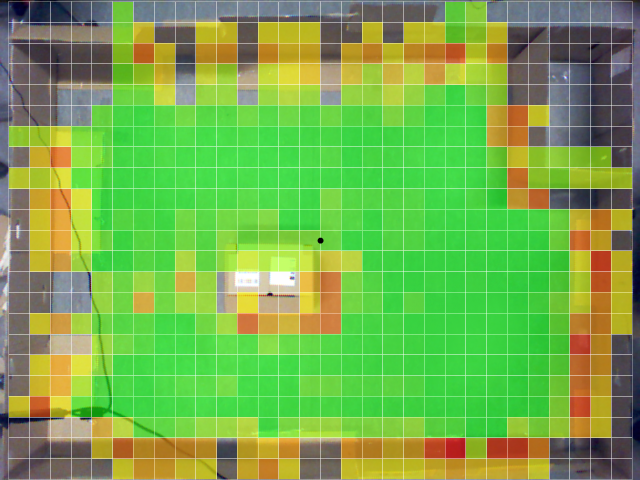
\includegraphics[width=\textwidth]{evaluering/gauss3_100.png}
		\end{column}
		\begin{column}{0.5\textwidth}
			\begin{itemize}
			\item \textbf{150}/150 opdateringer
			\item \textbf{337}/555 point
			\end{itemize}
			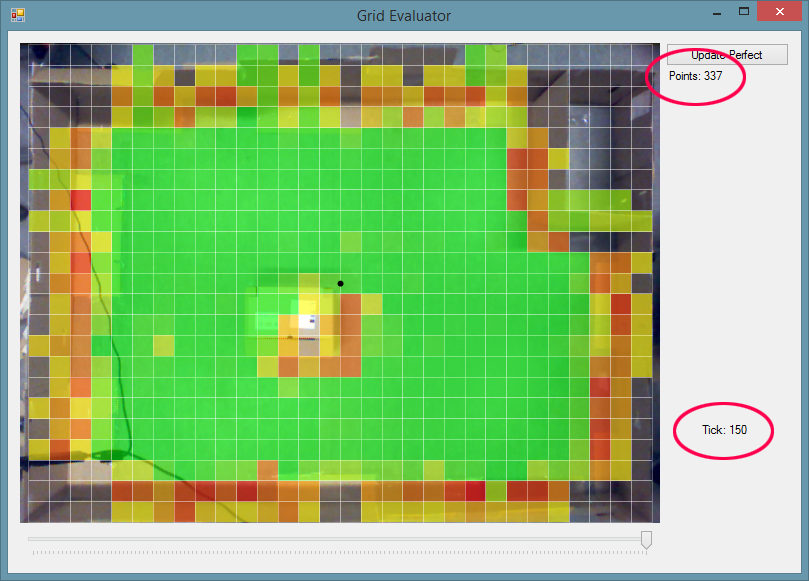
\includegraphics[width=\textwidth]{evaluering/gauss3_150.png}
		\end{column}
\end{columns}
\end{frame}

% SAMMENLIGNING AF SENSOR MODELLER
\begin{frame}[fragile]{Sammenligning af simpel- og gausisk sensormodel}
	\begin{columns}
		\begin{column}{0.5\textwidth}
			Simpel:
			\begin{itemize}
			\item \textbf{150}/150 opdateringer
			\item \textbf{193}/555 point
			\end{itemize}
			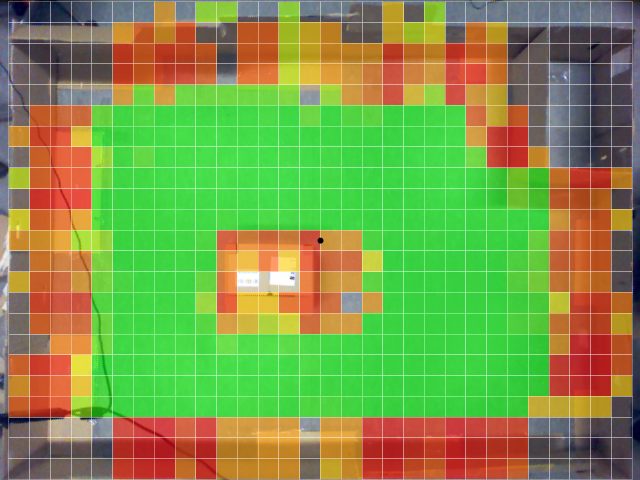
\includegraphics[width=\textwidth]{evaluering/simple3_150.png}
		\end{column}
		\begin{column}{0.5\textwidth}
			Gausisk:
			\begin{itemize}
			\item \textbf{150}/150 opdateringer
			\item \textbf{337}/555 point
			\end{itemize}
			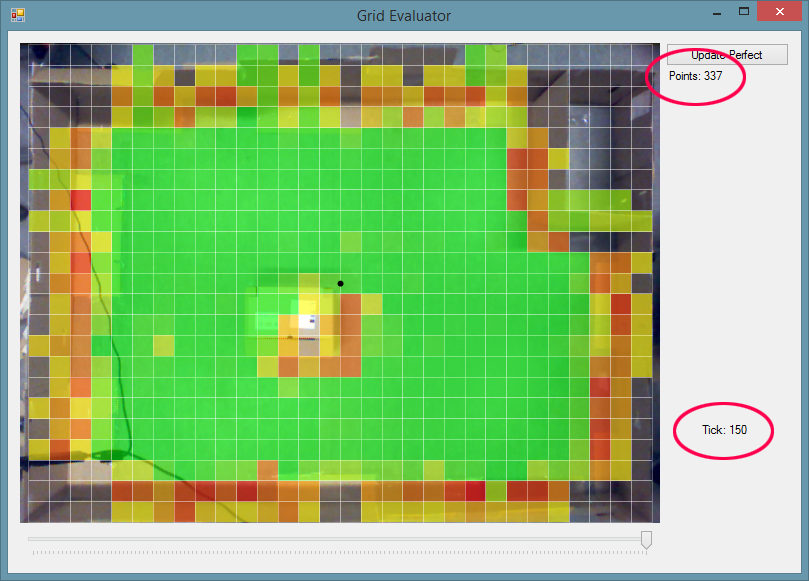
\includegraphics[width=\textwidth]{evaluering/gauss3_150.png}
		\end{column}
\end{columns}
\end{frame}

\subsection{Problemstillinger}

\begin{frame}
\frametitle{Punkter fra rapporten}
\begin{itemize}
\item Roterer og kører ikke præcist
\item Holder sig ikke altid indenfor den planlagte rute
\item Tager ikke højde for placering af sin bagende (og forende)
\item Sletter dele af kortet grundet forkerte sensormålinger
\item Uendelig løkke
\item Kører ind i forhindringer
\item Problemer med $90^\circ$ verden
\item Cellestørrelse
\item Gaussisk sensormodel i to dimensioner
\item Løbende målinger
\item Intet tårn
\item Robot bevist om egen størrelse og nærmeste omgivelser
\end{itemize}
\end{frame}


\subsection{Konklusion}

\begin{frame}
\frametitle{Konklusion}
\begin{itemize}
\item Problemformulering:\\
\textit{- Hvordan kan der konstrueres software til en robot, hvis formål er at kortlægge en ukendt verden, forudsat at den til enhver tid kender sin position?}
\pause
\item Robotten kortlægger en ukendt verden og anvender denne information til at navigere i verdenen.
\end{itemize}
\end{frame}